This section will give a broad overview of the whole System under development. It will explain how the System interacts with external systems and introduce its main functionality.

It will also describe the end users and the functionalities of the System reserved to them, detailing all the informations relevant to clarify their needs.

At last it will present the constraints and assumptions made for the System under development.

\subsection{Product Perspective}
This System will be implemented ex-novo to support all the functionalities required by the \textit{PowerEnJoy Car-Sharing Service}. It will be vastly built on top of the TCP/IP protocol, using a mix of HTTP and HTTP(S) as the main application protocols.

The System, for example, has to communicate with all the required external systems, such as the Banking System, needed to perform the monetary transactions, the Mailing System, which will forward the emails generated by the System, and the Mapping System, which is used in particular to show the GPS position of Cars, Users and Parking Areas on a map, check for existing addresses, and get the exact desired position in a specified address. In order to reach the objective, the System must use all the set of shared protocols and APIs.

Furthermore, the TCP/IP stack will also be used to communicate with the Cars and the different kind of Areas, in order to get all the meaningful information.
The System, for example, should be able to have access to all the informations provided by the wide variety of sensors placed inside the Cars, in order to know, in every moment, their GPS position, the status of their battery, their possible damages, their plugged status and the number of seats occupied. 
On the other hand, the System should also access data coming from a Charging or Parking Area (f.e. the number of free sockets and/or the number of free parking slots).

The interaction among the Users and the System will also be built using the Internet Protocol Suite. Users will access the System functionalities using the Application, which is the interface between the User and the back end of the System. The Application will use the HTTP(S) and TCP/IP protocols to allow the communication.

At last, Users should also be able to communicate their position to the System using their GPS coordinates. For this reason, the Application need access to the User GPS module, which is required in order to unlock previously reserved cars.

\subsubsection{Class Diagram}
The structure explained in the previous section is reported here using a Class Diagram.
\begin{figure}[h]
\centering
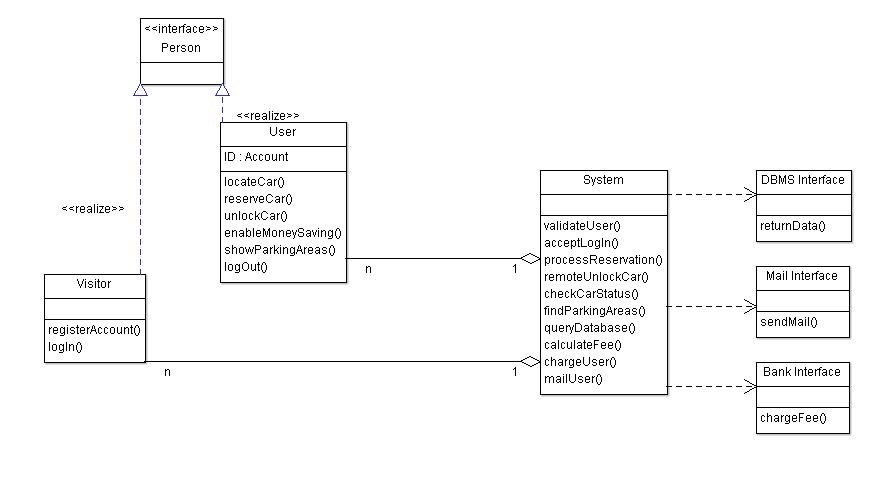
\includegraphics[width=\linewidth,keepaspectratio]{../Diagrams/CD/Class_Diagram.png}
\caption{Class Diagram}
\end{figure}
\FloatBarrier

\subsubsection{Statechart Diagram}
Here we have an UML Statechart diagram explaining the various states in which a Car can be.
\begin{figure}[h]
\centering
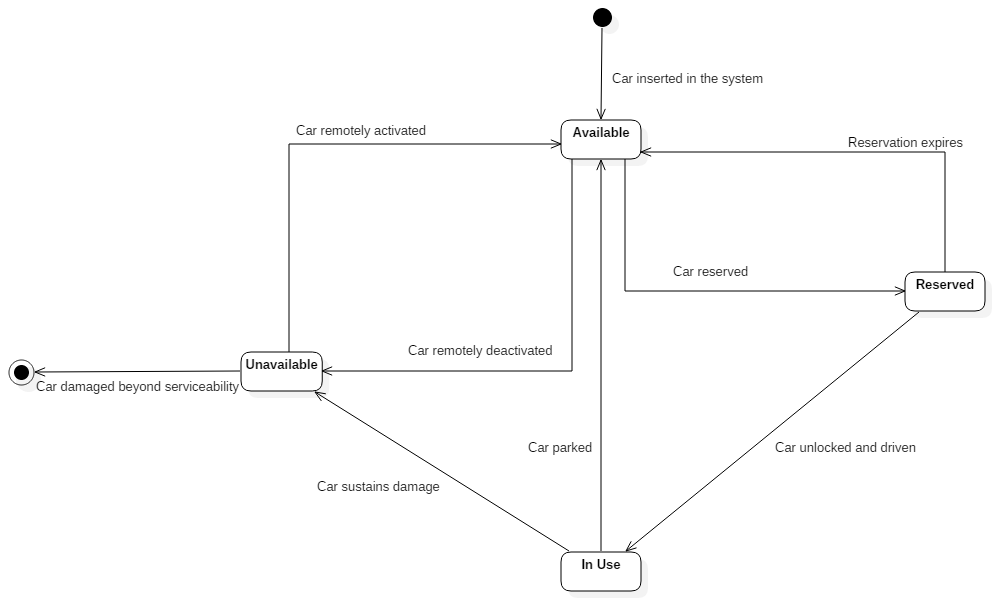
\includegraphics[width=\linewidth,keepaspectratio]{../Diagrams/SCD/SCD_Car.png}
\caption{Statechart diagram of Car}
\end{figure}
\FloatBarrier

\subsection{Product Functions}
Using the Application, the User will be able to register to the System. After a successful registration, the System will create an Account related to the User, which can use it to log in to the System and access the System functionalities.

The User can now use the Application to locate all the Cars, whose state is \textit{Available}, in two different ways: a) specifying a desired address or b) asking the System to locate him/her through the GPS coordinates. In the first case, the Mapping System is called to check for the existence of the specified address and to return a GPS position corresponding to that address. In both cases the GPS position will be sent to the Backend, which will return all the \textit{Available} Cars in a predefined distance range from the previously sent GPS position. The Mapping System will be called again by the Application to show to the User a map with all the Cars.

After locating the \textit{Available} Cars, the User can pick one of them and reserve it; at this moment, a one hour countdown starts during which the User will be able to unlock his/her reserved Car. If the User doesn't unlock the Car during the previous specified time period, the System cancels the reservation, sets the Car status as \textit{Available} and communicates to the Banking System the application of a fee.

The User can unlock the Car asking the System to locate him/her and if the Backend verifies that the User is in a specified distance range from the Car, the Car is unlocked and the User can now enter and drive it. During the drive, the System will display the Current Fee on the screen of the Car.

At the end of the ride, the System, basing on the time usage period of the Car, and on a set of bad or good behaviours, will evaluate the Fee and notify and the Banking System of the total amount to charge to the User's credit card.

\subsection{User Classes and Characteristics}
\begin{center}
  \begin{tabular}{|p{.2\textwidth}|p{.39\textwidth}|p{.39\textwidth}|}
    \hline
    \textbf{Name} & \textbf{Description} & \textbf{Actions} \\ \hline
    Visitor & A person who would like to register an account to access the System functionalities. & Can perform the registration and activation of the account. Successively he can log in the System becoming a User.\\\hline
    User & Someone who is registered in the System and can access its functionalities & Can locate, reserve and drive Cars. Will be charged for the use of the Cars. \\ \hline
    \end{tabular}
\end{center}
\vspace{5mm}
External access to the Database provided to Employees or any other person is under the responsibility and the regulations of the Company and is not managed by this System.

\subsection{Constraints}
\subsubsection{Hardware Constraints}\label{OE}
The Device used by the User should be able to establish an internet connection to the System using the Internet Protocol Suite. In addition, in order to perform the localization, reservation and unlocking of a Car the User device must have installed a working GPS module. 

The set of sensors, actuators and display inside Cars and Areas are already installed by the Company and the System has to communicate with them. Check the assumptions to see all the kind of hardware already shipped with Cars and Areas. 
On the other hand, the System will have a Car Board installed on each Car which will be used to enable the communication between the Car and the Backend. The aim is to avoid the constant polling of the Car sensors to get the data, using instead a special board to send the data only on specific events.

\subsubsection{Design and Implementation Constraints}
The System will employ the Internet Protocol Suite in order to enable the communication between its various parts, namely Application, Backend, Database and Car Board. The communication must be secured using at least the HTTP(S) application protocol.
The communication with the external systems will be built on top of the same set of protocols, accessing the API of this External Systems.

\subsection{Assumptions and Dependencies}
\begin{enumerate}
	\item The User do not create more than one Account at a time. Every User is accountable for improper use of their Account.
	\item Users will never forget their password.
	\item The User always provides real correct data in his/her registration form. 	
	\item The Company can decide at any time to revoke an User access to the System, charge the User with a fine or apply any other policy it choose (f.e. due to improper behaviour, unpaid bill, car parked outside a safe area, ...).
	\item The User which has reserved and then unlocked the Car will always be the person driving it. It will always be accounted for the usage of the Car and any improper action taken by the Driver. 
	\item The Database infrastructure in which the Cars, Parking Areas, Charging Areas, Users, etc, are stored, is owned and managed by the Company (and not by this System), which is responsible for its security, reliability and availability. Our System is provided by the Company with read/write access to the Database.
	\item The Company is responsible for the Employees and all their actions.
	\item The Car has a set of sensors that can detect, in every moment, its position, the status of its battery, the status of the engine, its damages, the connection of its plug to an electrical socket and the number of seats occupied. It also has actuators to remotely unlock its doors and a display to show information to the User. We assume that these devices are always perfectly functioning and their measures are always correct. In the case of damages to this devices, their repair is under the responsibility of the Company.
	\item After the doors of the cars are unlocked by the User, he/she always enters the Car, ignites the engine and leave the Parking Area.
	\item After a Car is Plugged to the Socket of a Charging Area, it will not be maliciously unplugged by the User himself/herself or by other people.
	\item An User can park/stop the Car everywhere and leave the Car at anytime. However, the system will not apply any fine only if he/she ends the ride inside a Parking or Charging Area. In all other cases the Company can decide to charge the User with a fine.
	\item If the Car has been left out of a Parking Area there will always be an Employee which immediately reaches it, recharges it and move it to a Charging Area. 
	\item When a User will park the Car inside a Parking or Charging Area, it will always correctly use one and only one free slot.		
	\item As soon as the Car battery status gets below 20\% of the full capacity AND the Car isn't in a Charging Area AND the Car Status isn't \textit{In Use} OR \textit{Plugged}, there's always an Employee that immediately reaches the Car and recharges it on site; in the meanwhile the Car status is \textit{Unavailable}.	
	\item When the Car is \textit{In Use} and the battery charge level reaches the 0\% of the full capacity the Car stops working.
	\item The Car will always be able to communicate a Major Damage to the System.
	\item If the Car status is \textit{Unavailable}, the Car will always be reached by an Employee to consider if the Car needs to be repaired, if an User should be charged for the damages or if the Car just needs to be recharged.
	\item A car which is \textit{Available} or \textit{Plugged} can be set as \textit{Unavailable} in every moment by an Employee. This is done through another Company's System as it is not provided in this System.
	\item A car which is \textit{Unavailable} can be set to \textit{Available} in every moment by an Employee. This is done through another Company's System and it is not provided in this System.
	\item Every fine received by the Company for improper use of the Car will be managed by the Company.
	\item Parking and Charging Areas have sensors to detect the number of parking and charging slots occupied at any time.
\end{enumerate}

\clearpage